\documentclass[12pt,a4paper,twoside]{article}

\usepackage[a4paper,left=2.2cm,right=2.2cm,bottom=2.5cm,top=2.5cm,footskip=32pt]{geometry}
\usepackage{setspace}
\usepackage{time}
\usepackage[sort]{natbib}
\usepackage{graphicx}
\usepackage{amsmath,amssymb,bm}
% \usepackage[dvipsnames]{xcolor}
\usepackage[table,xcdraw,dvipsnames]{xcolor}
\usepackage{hyperref}
\usepackage{multirow}
\usepackage{cleveref}

\usepackage{epigraph}
\setlength{\epigraphwidth}{2.9in}
\usepackage{authblk}
\newsavebox\CBox
\def\textBF#1{\sbox\CBox{#1}\resizebox{\wd\CBox}{\ht\CBox}{\textbf{#1}}}

\newcommand\myshade{85}
\colorlet{mylinkcolor}{violet}
\colorlet{mycitecolor}{YellowOrange}
\colorlet{myurlcolor}{Aquamarine}

\hypersetup{
	linkcolor  = mylinkcolor!\myshade!black,
	citecolor  = mycitecolor!\myshade!black,
	urlcolor   = myurlcolor!\myshade!black,
	colorlinks = true,
}

\usepackage{fancyhdr}
\usepackage[printwatermark]{xwatermark}
%\newwatermark[allpages,color=gray!50,angle=45,scale=1.5,xpos=0,ypos=0]{Draft. Do not circulate or cite}

\begin{document}%Data and Methods
	
\title{\normalsize{Extended abstract submitted to the International Population Conference 2021}\\
	\normalsize{\emph{Hyderabad, 5-10 December 2021}}\\
	$\,$\\	$\,$\\
	\begin{Huge}Forecasting vital rates from \\demographic summary measures\end{Huge}}


	\author[1]{Carlo G.~Camarda\thanks{Corresponding author: \url{carlo-giovanni.camarda@ined.fr}\\
		\hspace*{1.8em}Address: 9 cours des Humanités, 93322 Aubervilliers - France}}
\author[2]{Jos\'e Manuel Aburto}
\affil[1]{\small \textit{Institut national d'\'{e}tudes d\'emographiques (INED)}}
\affil[2]{\small \textit{Department of Sociology and Leverhulme Centre for Demographic Science,} \authorcr \textit{University of Oxford}}


\date{}
\maketitle
\thispagestyle{empty}

\pagestyle{fancy}
\fancyhead[RO,LE]{\small}
\fancyhead[LO]{\small Camarda \& Aburto: Forecasting vital rates from summary measures}% odd page header and number to right top
\fancyhead[RE]{\small Submitted to the IPC 2021}%Even page header and number at left top
\fancyfoot[L,R,C]{}
\rfoot{\thepage}

	
	
	\begin{abstract}
In population and actuarial sciences, time-trends of summary measures (such as life expectancy or the average number of children per woman) are easy to interpret and predict. Most summary measures are nonlinear functions of the vital rates, the key variable we usually want to estimate and forecast. Furthermore smooth outcomes of future age-specific vital rates are desirable. Therefore, optimization with nonlinear constraints in a smoothing setting is necessary. We propose a methodology that combines Sequential Quadratic Programming and a $P$-spline approach, allowing to forecast age-specific vital rates when future values of demographic summary measures are provided. We provide an application of the model on Italian mortality and Spanish fertility data.
\\
\\$\,$\\
{\bf Keywords:} Vital rates forecast; Smoothing; Constrained nonlinear optimization; Summary measures.
	\end{abstract}
	
%	\keywords{} 
	
	
	
	%%%%%--------------------------------------%%%%%%%%%%%%%%%%%%%
	%%%%%--------------------------------------%%%%%%%%%%%%%%%%%%%

	\newpage
	\pagenumbering{arabic} 
\setcounter{page}{1}	
\section{Introduction}\label{sec:Intro}

Future mortality and fertility levels can be predicted either by modelling and extrapolating rates over age and time, or by forecasting summary measures, later converted into age-specific rates. 
The latter approach takes advantage of the prior knowledge that demographers and actuaries have on possible future values of measures such as life expectancy at birth and total fertility rate. Among others, this methodology has been lately adopted by the United Nations \citep{SecikovaEtAlRates2016}. 
In this study, we propose a model to derive future mortality and fertility age-patterns complying with  projected summary measures. Unlike comparable approaches, we assume only smoothness of future vital rates, which is achieved by a two-dimensional $P$-spline approach as in \citep{CurrieDurbanEilersSmoothForecast2004}, and we allow constraints to multiple series of summary measures. Since these measures are commonly nonlinear functions of the estimated penalized coefficients, Lagrangian multipliers cannot be directly implemented. We hence opted for a Sequential Quadratic Programming (SQP) procedure \citep{NocedalWright2006} to perform the associated constrained nonlinear optimization.
We illustrate our approach with two data sets. We forecast mortality of Italian females, based on future life expectancy predicted by \citet{WPP2019} and a future trend of a lifespan disparity measure obtained by time-series analysis. We also forecast Spanish fertility constrained to future values of total fertility rates, mean and variance of age at childbearing, derived by time-series analysis.

\section{Model on Italian mortality data}

For ease of presentation, we formulate the model on mortality data. We suppose that we have deaths, and exposures to risk, arranged in two matrices, 
$\bm{Y} = (y_{ij})$ and $\bm{E} = (e_{ij})$, each $m \times n_{1}$, whose rows and columns are classified by age at death, $\bm{a}, \,m \times 1$, and year of death, $\bm{t}_{1}, \,n_{1} \times 1$, respectively.  
We assume that the number of deaths $y_{ij}$ at age $i$ in year $j$ is Poisson distributed with mean $\mu_{ij} \,e_{ij}$. %The value of $\mu_{ij}$ is commonly named force of mortality. 
Forecasting aims to reconstruct trends in $\mu_{ij}$ for $n_{2}$ future years, $\bm{y}_{2}, n_{2} \times 1$.

It is common practice to summarize mortality age-patterns by computing measures such as life expectancy at birth ($e_{0}$) and lifespan disparity measures. Time-trends of these summary measures are often regular and well-understood. Forecasting these time-series is therefore an easier task. Figure~\ref{fig:CamardaMort} (top-left panel) presents observed $e_{0}$ for Italian females from 1960 to 2016 along with the medium variant up to 2050 as computed by the UN. A second constraint is given by future values of $e^{\dagger}$, a lifespan disparity measure defined as the average years of life lost in a population attributable to death \citep{VaupelCRdemo2003}. Future values of this measure are obtained by conventional time-series models and portrayed in the top-right panel of Figure~\ref{fig:CamardaMort}. Future mortality patterns, both by age and over time, must adhere to these predicted trends.

\begin{figure}[!ht]\centering
	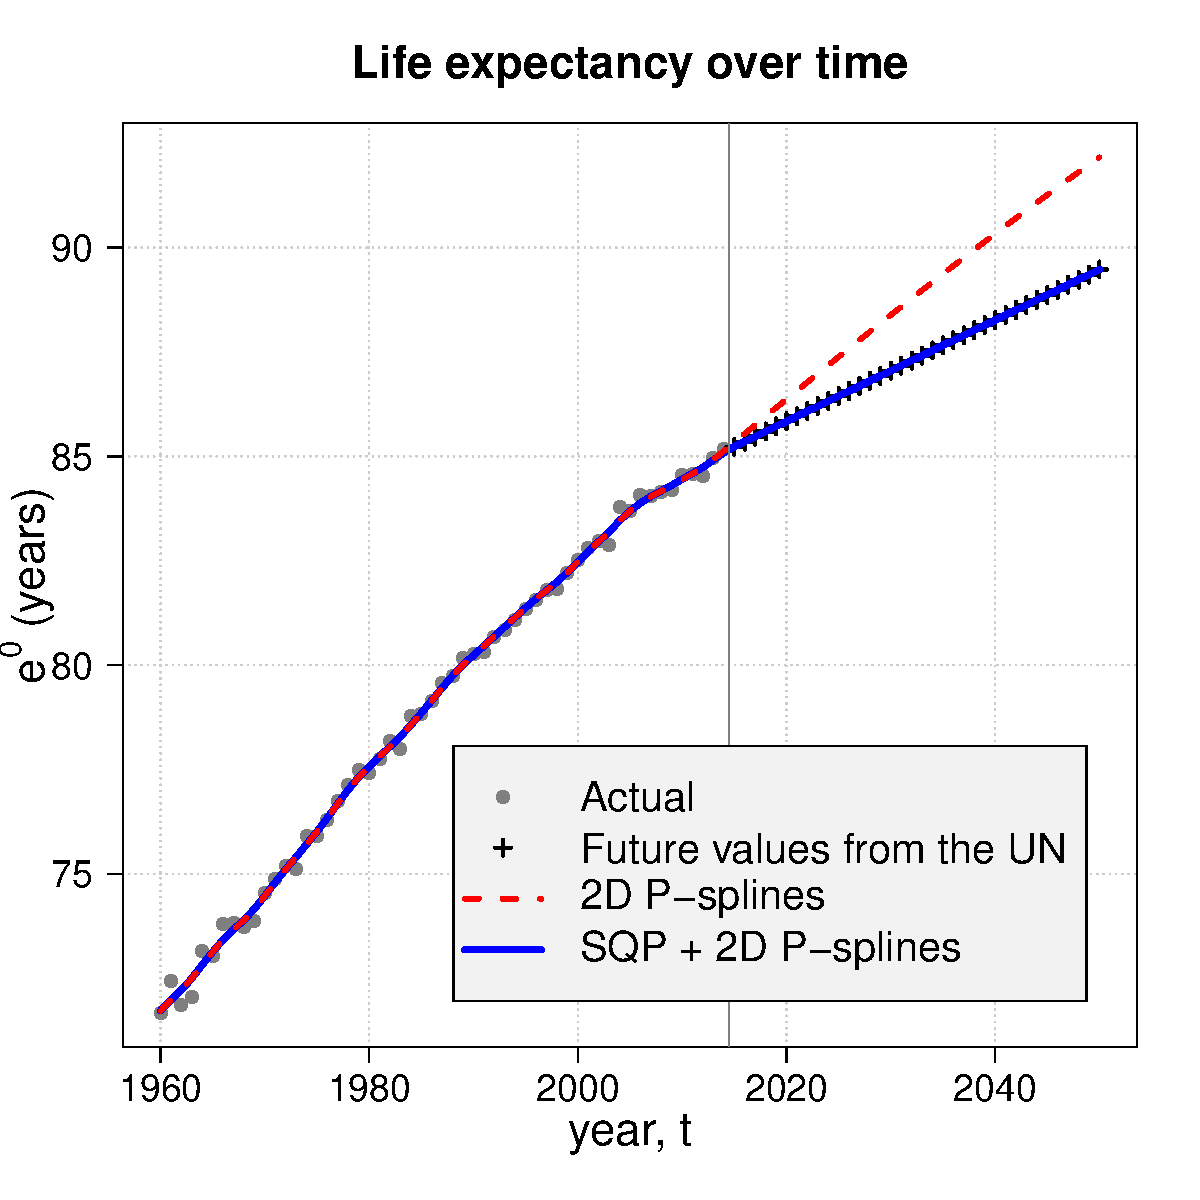
\includegraphics[scale=0.35]{./Figures/Camardafig1a.pdf}
	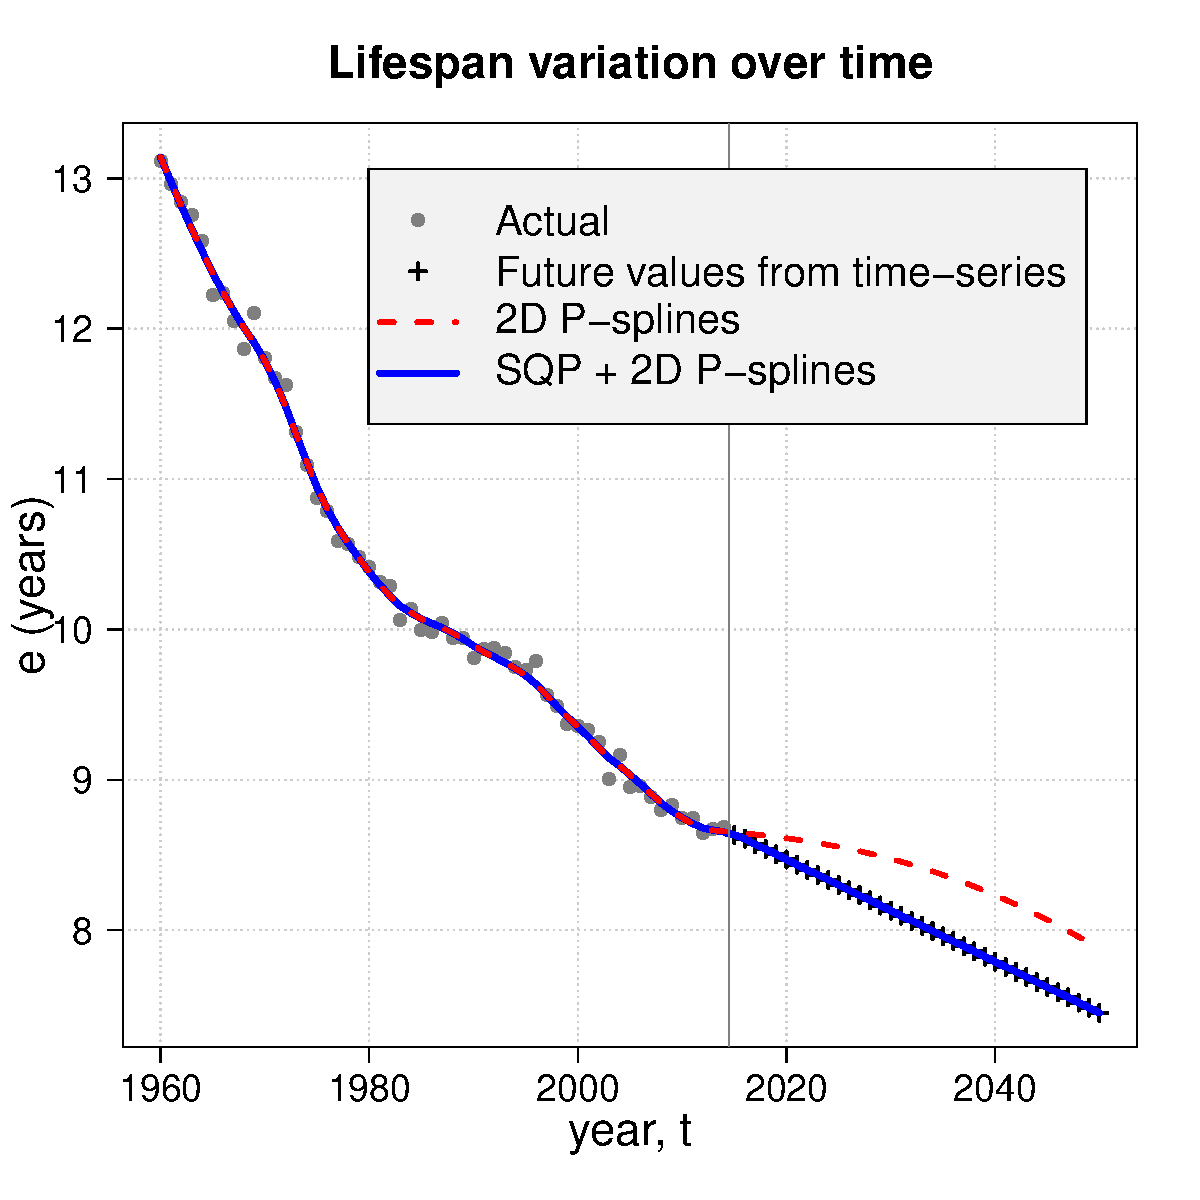
\includegraphics[scale=0.35]{./Figures/Camardafig1b.pdf}
	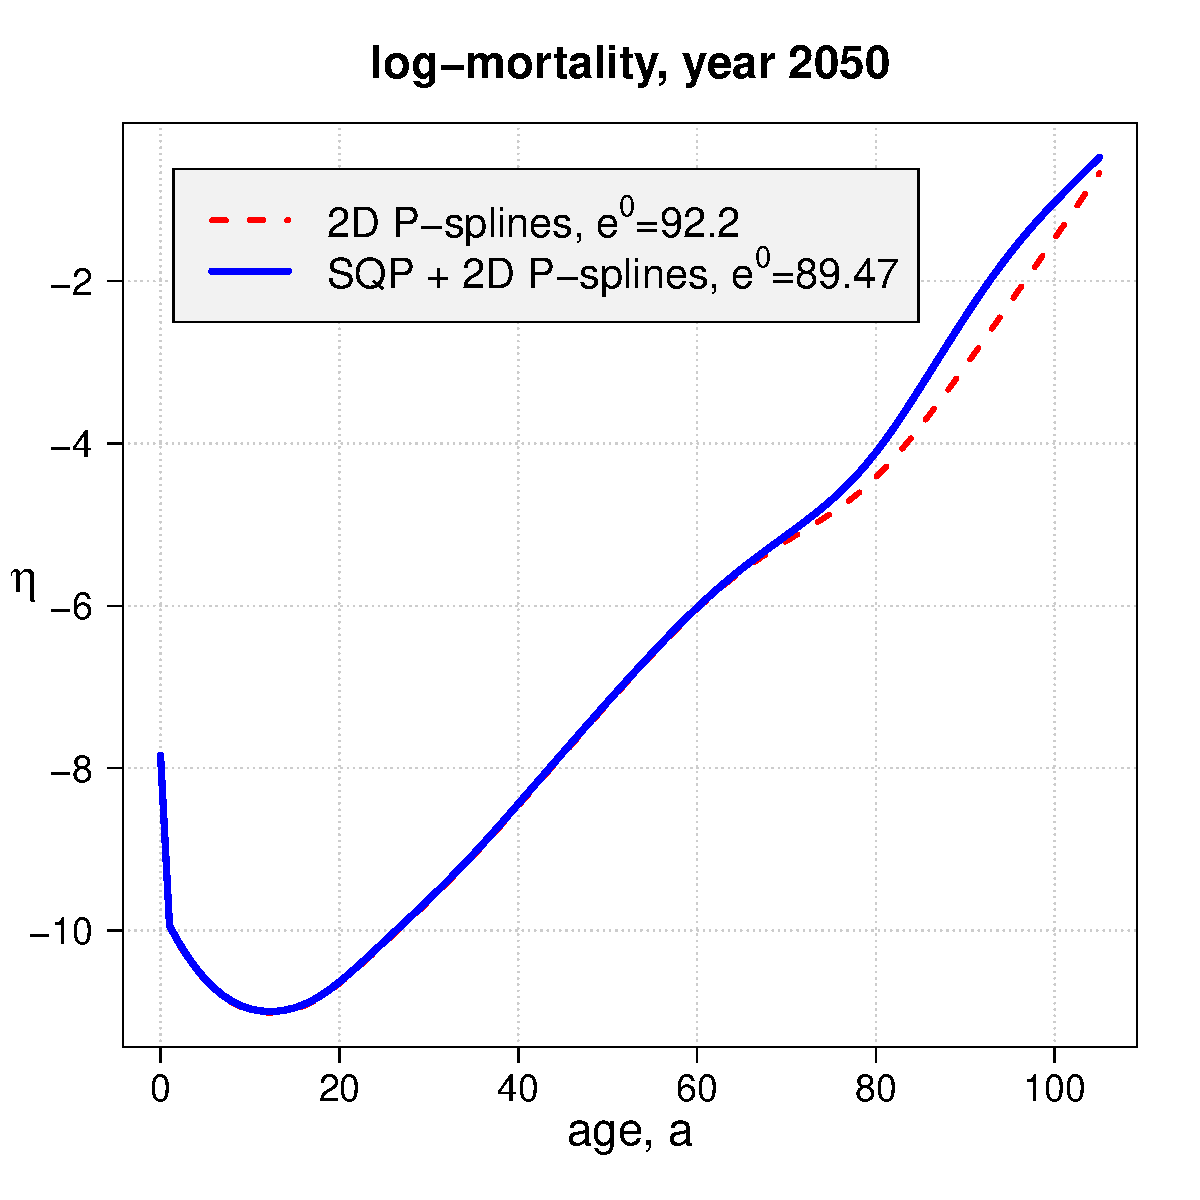
\includegraphics[scale=0.35]{./Figures/Camardafig1c.pdf}
	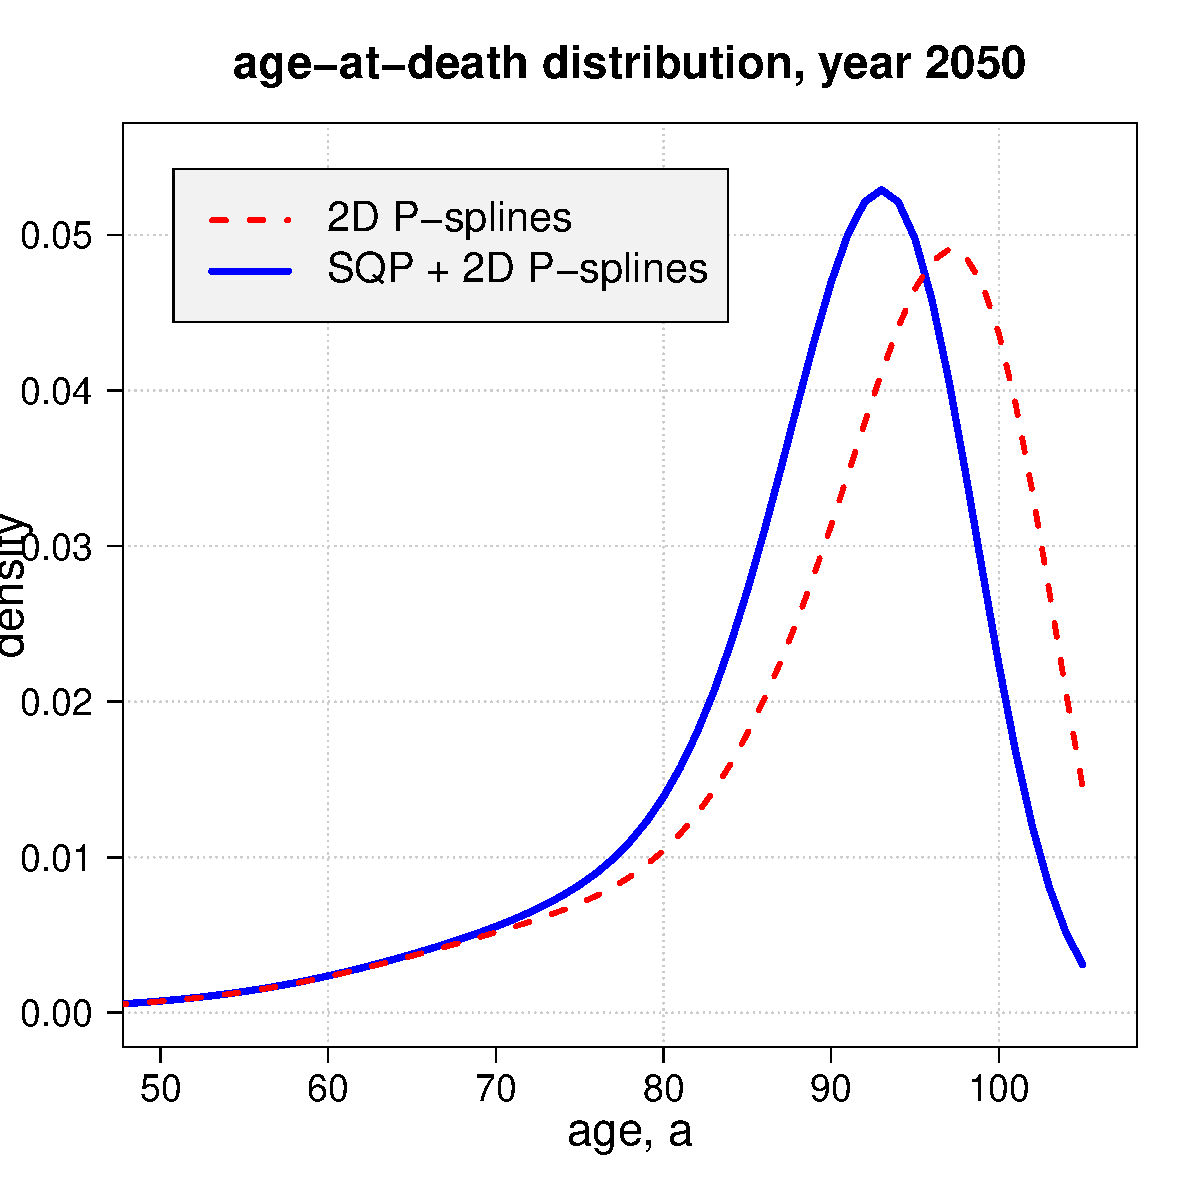
\includegraphics[scale=0.35]{./Figures/Camardafig1d.pdf}
	\caption{\label{fig:CamardaMort} Top panels: Actual, estimated and forecast life expectancy at birth and lifespan disparity measure by United Nations and time-series, 2D $P$-splines and the SQP+2D $P$-splines. Bottom panels: Mortality in 2050 described by log-hazards and associated densities (ages 50+) by 2D $P$-splines and the SQP+2D $P$-splines. Italian females, ages 0-105, years 1960-2014, forecast up to 2050.}
\end{figure}

We arrange data as a column vector, that is, $\bm{y} = \verb"vec"(\bm{Y})$ and $\bm{e} = \verb"vec"(\bm{E})$ and we model our Poisson death counts as follows: $\ln(E(\bm{y})) = \ln(\bm{e})+ \bm{\eta} = \ln(\bm{e})+ \bm{B}\,\bm{\alpha}\, , $ where $\bm{B}$ is the regression matrix over the two dimensions: $\bm{B} = \bm{I}_{n_{1}} \otimes \bm{B}_{a}$, with $\bm{B}_{a} \in \mathbb{R}^{m \times k_{a}}$. Over time, we employ an identity matrix of dimension $n_{1}$ because we will incorporate a constraint for each year. Over age, $\bm{B}_{a}$ includes a specialized coefficient for dealing with mortality at age 0. In order to forecast, data and bases are augmented as follows:
\begin{equation}\label{eq:AugData}
\breve{\bm{E}} = [\bm{E} : \bm{E}_{2}]\, , \qquad 
\breve{\bm{Y}} = [\bm{Y} : \bm{Y}_{2}]\, , \qquad
\breve{\bm{B}} = \bm{I}_{n_{1}+n_{2}} \otimes \bm{B}_{a}
\, ,
\end{equation}
where $\bm{E}_{2}$ and $\bm{Y}_{2}$ are filled with arbitrary future values. If we define a weight matrix $\bm{V} = \mathrm{diag}(\verb"vec"(\bm{1}_{m\times n_{1}}:\bm{0}_{m\times n_{2}}))\,$, the coefficients vector $\bm{\alpha}$
can be estimated by a penalised version of the iteratively reweighted least squares algorithm: 
\begin{equation}\label{eq:penIRWLSfor}
(\breve{\bm{B}}' \bm{V} \tilde{\bm{W}} \breve{\bm{B}} + \bm{P}) \tilde{\bm{\alpha}} =
\breve{\bm{B}}'\bm{V} \tilde{\bm{W}}\tilde{\bm{z}} \, ,
\end{equation} 	
where a difference penalty $\bm{P}$ enforces smoothness behaviour of mortality both over age and time. Outcomes from this approach in terms of life expectancy and $e^{\dagger}$ are depicted with a dashed line in Figure~\ref{fig:CamardaMort} (top panels), and departures from the UN and time-series projected values are evident. 

Both life expectancy and average years of life lost are nonlinear function of the coefficients vector $\bm{\alpha}$. For a year $j$ and associated $k_{a}$ coefficients $\bm{\alpha}_{j}$, we denote mortality by $\bm{\mu}_{j} = \exp(\bm{B}_{a}\bm{\alpha}_{j})$. We can write our summary measures as follows
\begin{eqnarray}\label{eq:e0ed}
e^{0} (\bm{\alpha}_{j}) &=& \;\;\,\,\bm{1}_{m}' \, \exp[ \bm{C} \, \bm{\mu}_{j}]  + 0.5 \\
e^{\dagger} (\bm{\alpha}_{j}) &=&  - \exp[ \bm{C} \, \bm{\mu}_{j}]' \, \bm{C} \bm{\mu}_{j} \nonumber
\end{eqnarray} 
where $\bm{C}$ is a $(m \times m)$ lower triangular matrix filled only with -1. 

%\begin{equation}\label{eq:Cmat}
%\bm{C} = \left[\begin{array}{rrrr}
%-1 & 0 & \cdots & 0 \\
%-1 & -1& \cdots & 0 \\
%\vdots & \vdots & \ddots & \vdots \\
%-1 & -1 & \cdots & -1
%\end{array}\right] \, .
%\end{equation}

Constrained nonlinear optimization is therefore	necessary and a SQP approach is implemented. Let denote with $\bm{N}^{0}$ and $\bm{N}^{\dagger}$ the $(k_{a}n_{2} \times n_{2})$ matrices with block-diagonal structures containing derivatives of~\eqref{eq:e0ed} with respect to $\bm{\alpha}_{j}$ for $j=n_{1}+1, \ldots n_{1}+n_{2}$:
\begin{eqnarray}\label{eq:Der}
\frac{\partial e^{0} (\bm{\alpha}_{j})}{\partial \bm{\alpha}_{j}} &=& \bm{1}_{m}' \verb"diag"[\exp(\bm{C}\bm{\mu}_{j})] \,	\bm{C} \,\verb"diag"(\bm{\mu}_{j}) \bm{B}_{a}\\
\frac{\partial e^{\dagger} (\bm{\alpha}_{j})}{\partial \bm{\alpha}_{j}} &=& - \bm{B}_{a}' \left\{ \bm{C}'[\bm{C}\bm{\mu}_{j} \circ \exp(\bm{C}\bm{\mu}_{j})] \circ \bm{\mu}_{j} \right\} + \nonumber\\
&& - \bm{B}_{a}' \left\{ [\bm{C}' \exp(\bm{C}\bm{\mu}_{j})] \circ \bm{\mu}_{j} \right\} \nonumber\, ,
\end{eqnarray}
where $\circ$ represents element-wise multiplication. Target life expectancy and lifespan disparity for future years are given by $n_{2}$-vectors $\bm{e}^{0}_{\mathrm{T}}$ and $\bm{e}^{\dagger}_{\mathrm{T}}$.

Solution of the associated system of equations at the step $\nu + 1$ is given by
\begin{equation}\label{eq:SQLalg}
\left[ \begin{array}{l}
\bm{\alpha}_{\nu+1}\\
\bm{\omega}_{\nu+1}
\end{array}\right] = 
\left[ \begin{array}{lllll}
\bm{L}_{\nu}  &:& \bm{H}^{0}_{\nu} &:& \bm{H}^{\dagger}_{\nu}\\
\bm{H}_{\nu}^{0 T}  &:& \bm{0}_{n_{2} \times n_{2}}&:&\bm{0}_{n_{2} \times n_{2}}\\
\bm{H}_{\nu}^{\dagger T} &:& \bm{0}_{n_{2} \times n_{2}} &:& \bm{0}_{n_{2} \times n_{2}}
\end{array}\right]^{-1}
\left[ \begin{array}{c}
\bm{r}_{\nu} - \bm{L}_{\nu}\bm{\alpha}_{\nu}\\
\bm{e}^{0}_{\mathrm{T}} - \bm{e}^{0} (\bm{\alpha}_{\nu})\\
\bm{e}^{\dagger}_{\mathrm{T}} - \bm{e}^{\dagger} (\bm{\alpha}_{\nu})\\
\end{array}\right] \, ,
\end{equation}
where $\bm{L}$ and $\bm{r}$ are left- and right-hand-side of the system in~\eqref{eq:penIRWLSfor}, and matrices $\bm{H}^{0} = \left[\bm{0}_{k_{a}n_{1}\times n_{2}}:\bm{N}^{0} \right]'$ and $\bm{H}^{\dagger} = \left[\bm{0}_{k_{a}n_{1}\times n_{2}}:\bm{N}^{\dagger} \right]'$. Vector of $\bm{\omega}$ denotes the current solution of the associated Lagrangian multipliers for both set of constraints.

Future values for $e^{0}$ and $e^{\dagger}$ forecast by the proposed method are exactly equal to the UN and time-series values (Figure~\ref{fig:CamardaMort}, top panels). The bottom panels show the forecast mortality age-pattern in 2050: the shape obtained by the suggested approach is not a simple linear function of the plain $P$-splines outcome, and differences are evident by looking at the associated age-at-death distributions. 

\section{Spanish Fertility Data}

We forecast Spanish fertility using three commonly-used summary measures: Total Fertility Rate describing average number of children per women in a given year, and mean and variance of childbearing age which measure fertility shape over age. In formulas:
\begin{eqnarray}\label{eq:FertMea}
TFR(\bm{\alpha}_{j}) &=& \bm{1}_{m}' \, \bm{\mu}_{j}\\
MAB(\bm{\alpha}_{j}) &=& \bm{\mu}_{j}' \, (\bm{a}+0.5) \; / \; TFR(\bm{\alpha}_{j})\nonumber\\
VAB(\bm{\alpha}_{j}) &=& \bm{\mu}_{j}' \, (\bm{a}+0.5)^2 \; / \; TFR(\bm{\alpha}_{j}) - MAB(\bm{\alpha}_{j})^2\nonumber \, .
\end{eqnarray} 

We forecast trends of these measures by time-series analysis. We then smooth and constrain future fertility age-patterns to comply forecast values of \eqref{eq:FertMea} as in \eqref{eq:SQLalg}. Summary measures as well as fertility rates in 2050 are presented in Figure~\ref{fig:CamardaFert}. Differences between proposed approach and plain 2D $P$-splines are clear. Whereas $P$-splines blindly extrapolate previous trends mainly accounting for the last observed years, the proposed approach enforces future age-patterns to adhere combinations of summary measures, guiding future fertility toward demographic meaningful trends. 

\begin{figure}[!ht]\centering
	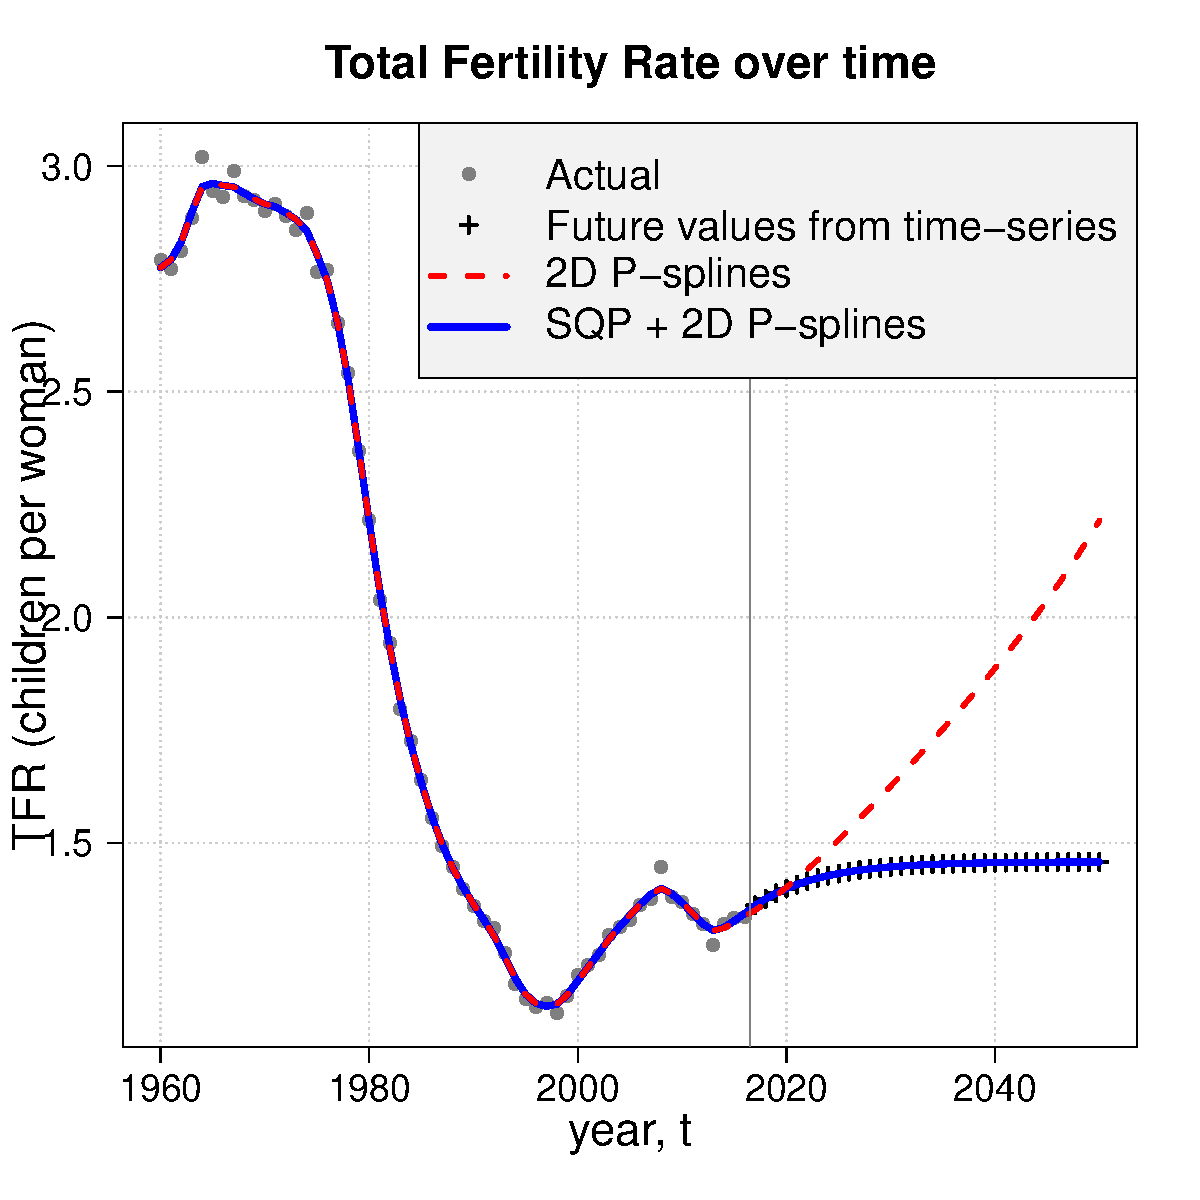
\includegraphics[scale=0.35]{./Figures/Camardafig2a.pdf}
	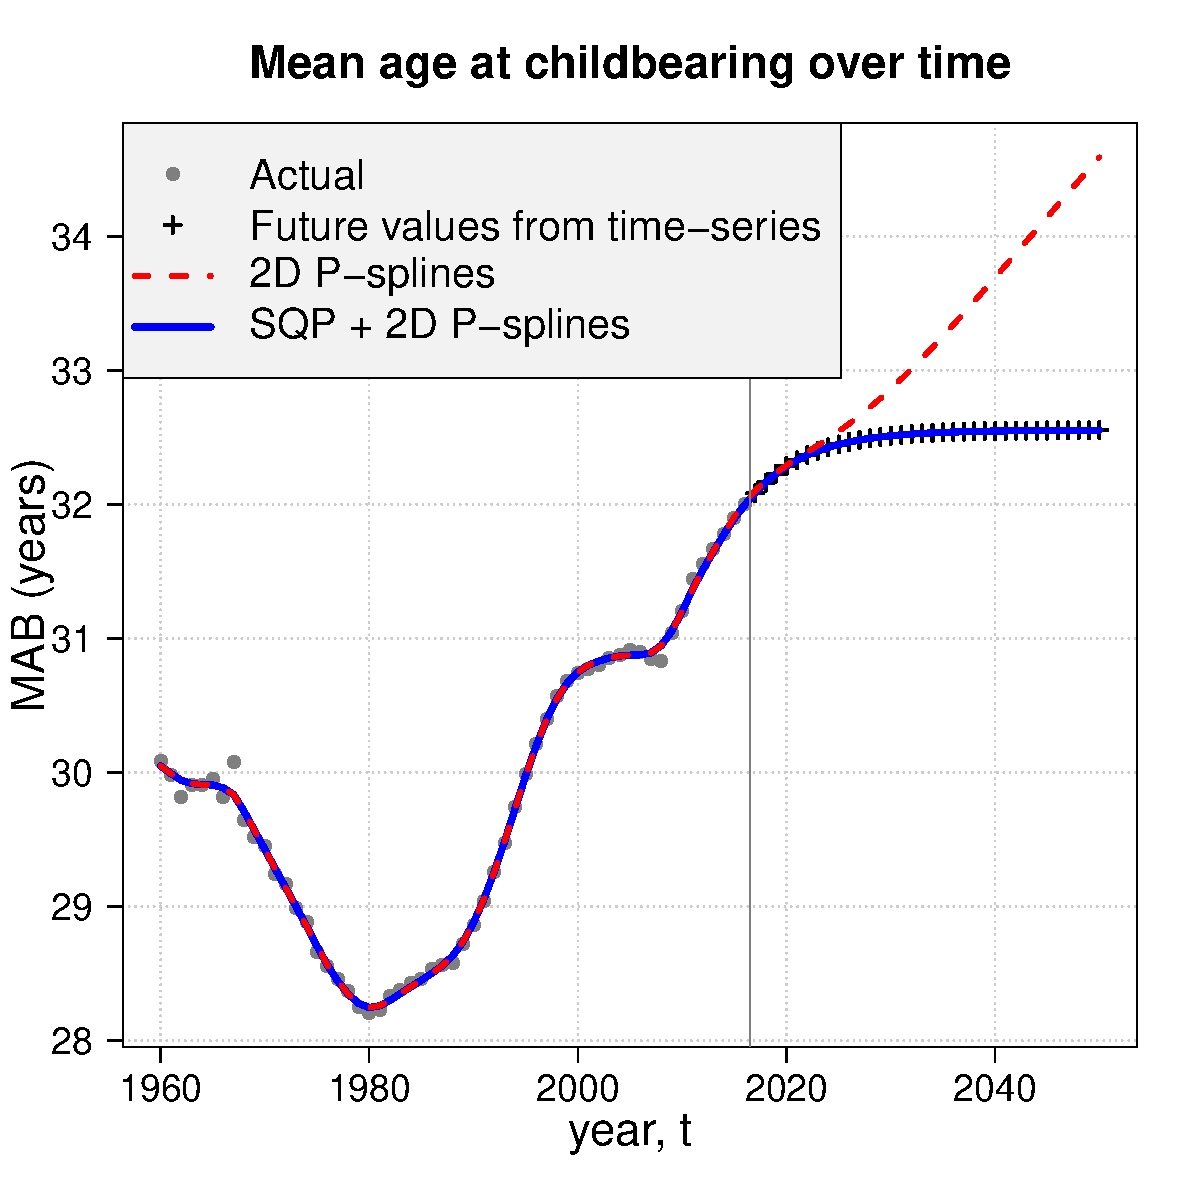
\includegraphics[scale=0.35]{./Figures/Camardafig2b.pdf}
	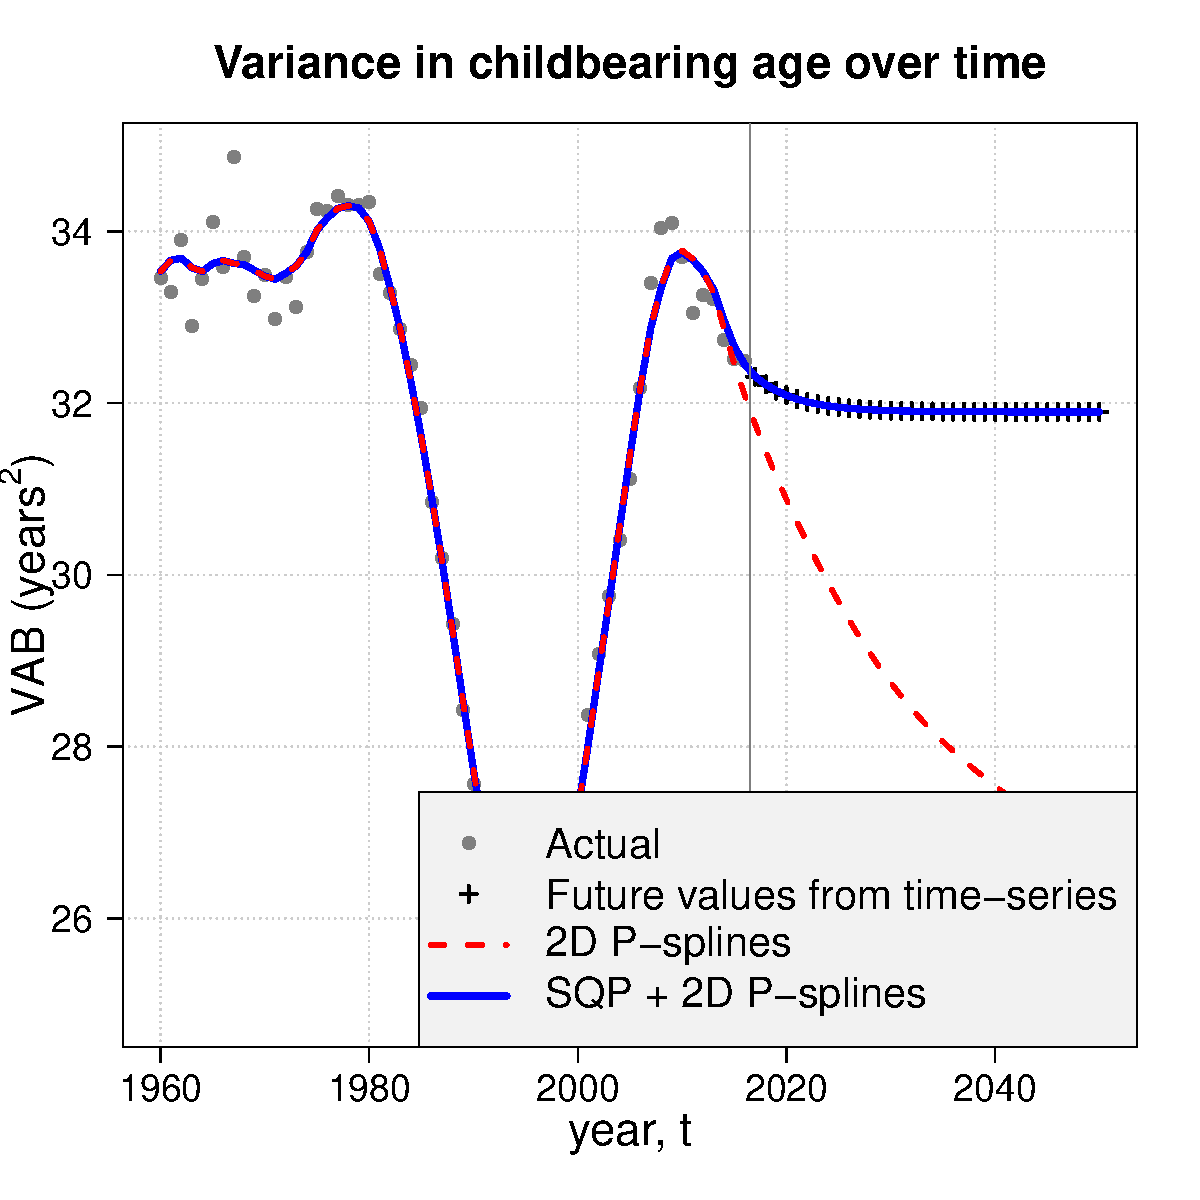
\includegraphics[scale=0.35]{./Figures/Camardafig2c.pdf}
	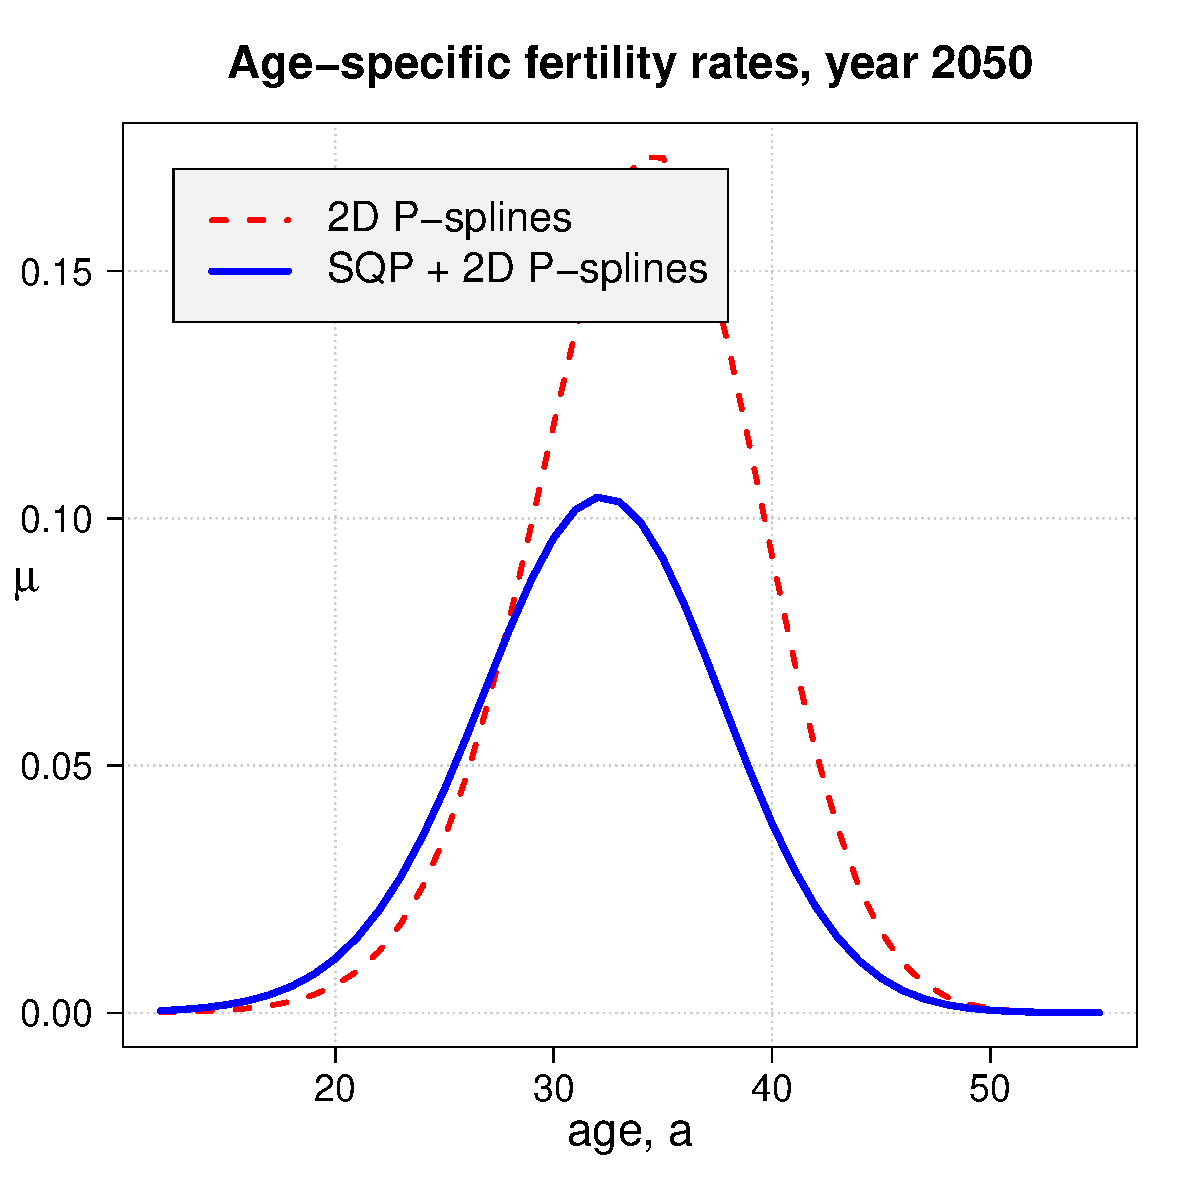
\includegraphics[scale=0.35]{./Figures/Camardafig2d.pdf}
	\caption{\label{fig:CamardaFert} Top and left-bottom panels: Actual, estimated and forecast Total Fertility Rate, Mean and Variance in childbearing age by time-series analysis, 2D $P$-splines and the SQP+2D $P$-splines. Right-bottom panel: Age-specific fertility rate in 2050 by 2D $P$-splines and the SQP+2D $P$-splines. Spain, ages 12-55, years 1960-2016, forecast up to 2050.}
\end{figure}

\section{Concluding remarks}

In this study, we combine smoothing models ($P$-splines) and optimization with nonlinear constraints (Sequential Quadratic Programming) to forecast vital rates when future values of demographic summary measures are provided. 
%The proposed approach allows to obtain smooth future mortality and fertility patterns which comply projected measures commonly easy to interpret and predict. 

We envisage further applications. Forecast of vital rates for partially completed cohorts is often relevant in population studies. For instance, final fertility history of a given cohort may be hypothesized though age-pattern is not yet observed and its estimation will be necessary. We also plan to adopt our approach to reconstruct demographic scenarios which are conventionally based on summary measures. 

From a methodological perspective, future work will be realized to incorporate uncertainty and to objectively select the amount of smoothness in future mortality and fertility age-patterns.


\newpage
\thispagestyle{empty}
\bibliographystyle{chicago}
\bibliography{bibliografia1}
	
\end{document}